\chapter{Inleiding}
\label{inleiding}

\section{Algemene context}

Wetenschappelijke vooruitgang heeft ervoor gezorgd dat de kost om genomen te sequencen het afgelopen decennium exponentieel gedaald is, sinds 2008 zelfs aan een hogere snelheid dan de evolutie volgens de wet van Moore \cite{wetterstrand_sequencing_cost}. Dit is duidelijk zichtbaar op de grafiek in figuur \ref{sequencing_cost}. In allerhande soorten biologisch, medisch en pharmaceutisch onderzoek worden dan ook genomen van meer en meer organismen gesequencet en dit genereert enorme hoeveelheden data. Ter illustratie: de \textit{whole genome sequencing pipeline} van het Broad Institute \cite{broad_institute}, een referentie in het veld, genereert bij het sequencen van 1 volledig menselijk genoom in de orde van 3TB aan tussentijdse data. Het eindresultaat is 50 GB gecomprimeerde data voor 1 menselijk genoom bij 50x \textit{coverage} (een maat voor de resolutie \cite{coverage_definition}). Naarmate genomen van miljoenen mensen en andere levende wezens geanalyseerd en opgeslagen worden, vereist deze evolutie steeds betere schaalbaarheid, responstijd, en parallellisering voor de opslag en verwerking van deze data.\\

Een logische stap is om deze problemen aan te pakken met grote verdeelde computersystemen, zogenaamde \textit{high performance computing systems} of \textit{supercomputers}. Het Exascience Life Lab van imec, Intel, Janssen Pharmaceutica en de 5 Vlaamse universiteiten verricht specifiek onderzoek naar de toepassing van supercomputers om het genoomsequencingproces te versnellen \cite{lifelab_bwa}\cite{exascience_life_lab}.\\
De snel toegenomen populariteit van webdiensten als sociale netwerken zadelde webservice-leveranciers op met een gelijkaardige explosie aan data. Om deze zogenaamde Big Data \cite{mashey1997big} adequaat te beheren, volstaan traditionele relationele DBMS niet meer. Daarom hebben grote webbedrijven zoals Google, Amazon en Facebook nieuwe opslagtechnieken ontwikkeld die voldoen aan de vereisten qua incrementele schaalbaarheid, lage responstijden en hoge beschikbaarheid \cite{baker2011megastore}. Dit heeft vele zogenaamde NoSQL ('Not only SQL') databases voortgebracht, die het rigide relationele datamodel inruilen voor betere schaalbaarheid en gemakkelijkere distributie van de data. Daarnaast is er ook de recentere opkomst van NewSQL-systemen: deze trachten de schaalbaarheid, distributie en fouttolerantie van NoSQL-systemen te combineren met het relationele datamodel en de bijhorende SQL-query interface en sterke garanties op gebied van concurrency en consistentie.

\begin{figure}[h!]
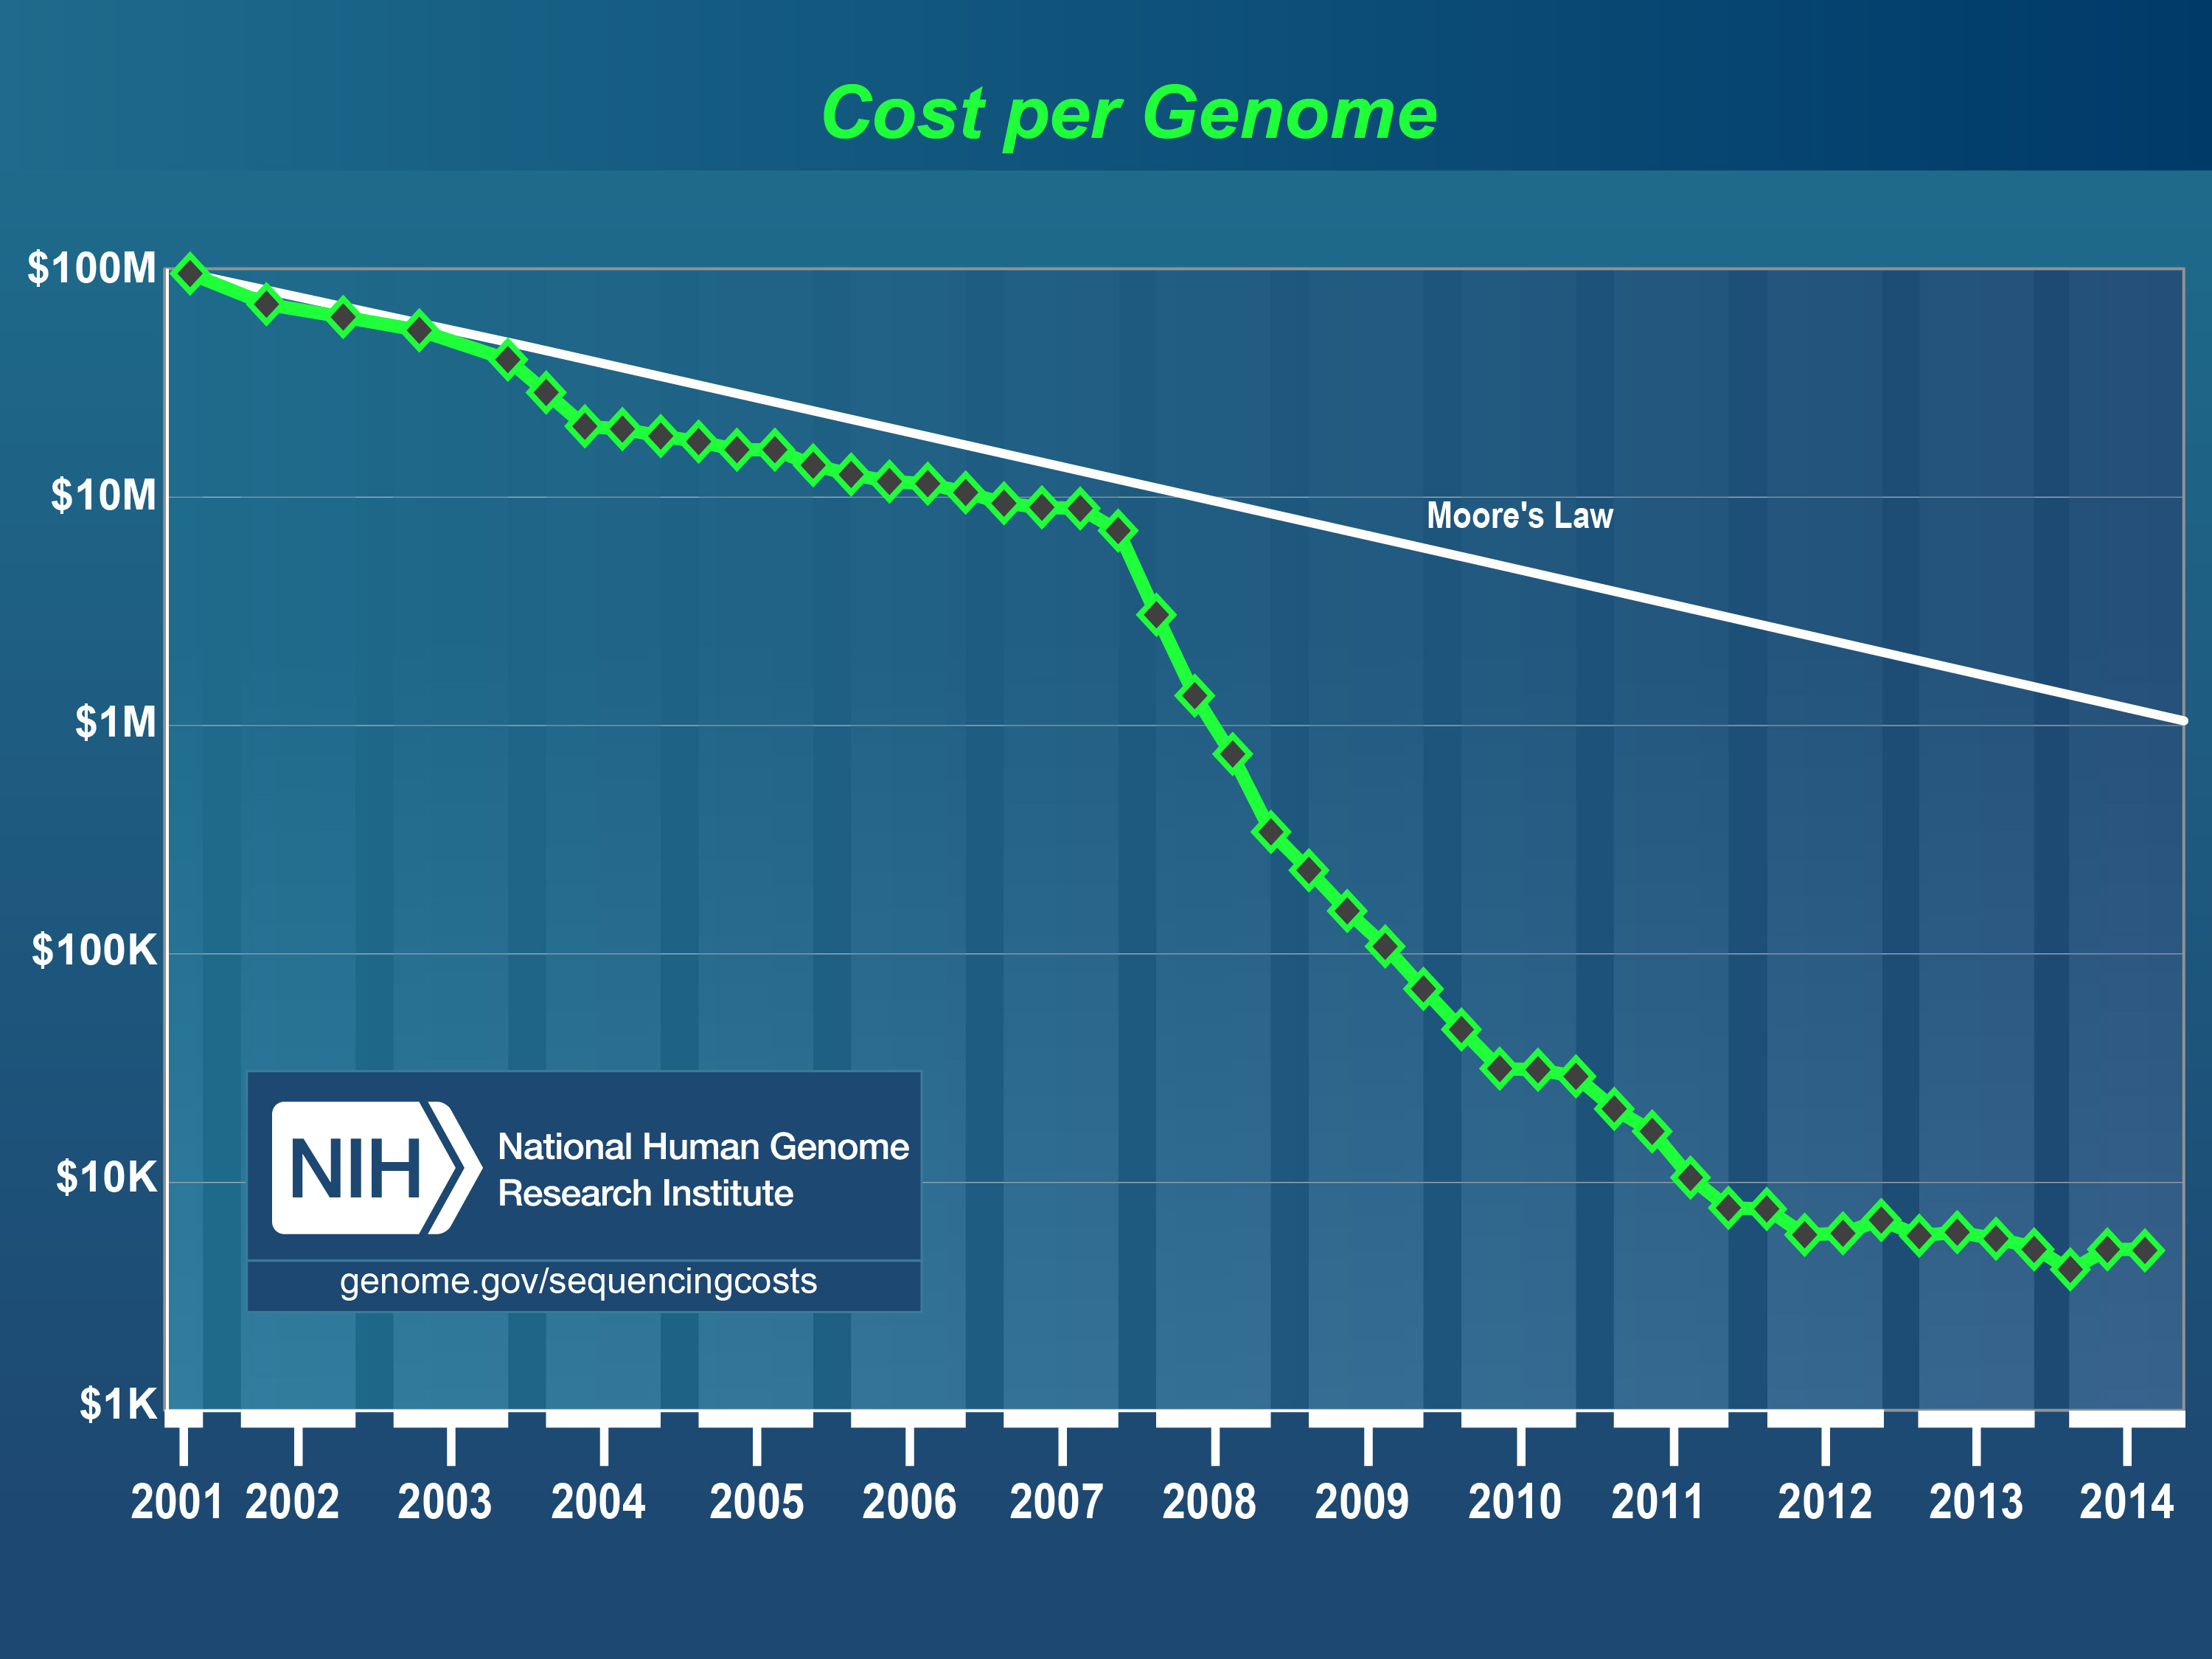
\includegraphics[width=\textwidth,height=\textheight,keepaspectratio]{cost_genome}
\caption{Evolutie van de prijs om een genoom te sequencen sinds 2001}
\label{sequencing_cost}
\end{figure}

\section{Probleemstelling case study: GEMINI}

Een concreet voorbeeld van genoomanalyse-infrastructuur die door de hierboven beschreven sequencing-boom tegen haar grenzen botst, is GEMINI. Op vraag van Janssen Pharmaceutica bestudeert deze thesis als case study deze genoomanalysetool. GEMINI (van GEnome MINIng) is een software-framework voor flexibele analyse van genetische variaties in grote datasets van genomen, ontwikkeld aan de University of Utah \cite{10.1371/journal.pcbi.1003153}. Deze datasets aan genomen bevatten informatie over de genetische \textit{variants} - d.w.z. stukken van genen zoals deze in het genoomsequencingproces waargenomen worden, van meerdere proefpersonen (ook: \textit{samples}). GEMINI vertrekt daarbij van VCF(Variant Call Format)-bestanden: dit zijn tekstbestanden die informatie over het gesequencete DNA van de samples bevatten, op het niveau van individuele variants. GEMINI laadt deze gegevens in in een database, voegt allerlei annotaties toe met bijkomende informatie van enkele vermaarde onderzoeksinstituten, en biedt dan de mogelijkheid queries uit te voeren op deze databank. GEMINI laat de gebruiker ook toe zelfgedefinieerde annotaties toe te voegen aan de variants. \\
De huidige operationele versie van GEMINI draait op de eenvoudige SQL-databank SQLite, maar deze laat op gebied van schaalbaarheid en performantie te wensen over. De gewenste schaalbaarheid ligt in 2 dimensies: enerzijds het aantal variants in de dataset, en anderzijds het aantal samples wier DNA in de dataset geanalyseerd wordt. Bij toenemend 
%TODO getal!
aantal samples of variants duurt zowel het inladen van de genoomdata in de databank voor als het queryen tijdens effectief gebruik te lang om gebruiksvriendelijk te zijn. Het inladen van de genoomdata uit VCF-files is, enigszins contra-intu\"itief, geen eenmalige of zeldzame operatie: de huidige productieversie van GEMINI laat niet toe om na het inladen nog samples of variants toe te voegen, met als gevolg dat bij elke iteratie van een genetisch of biologisch experiment die nieuwe informatie oplevert, de volledige dataset opnieuw ingeladen dient te worden. Ook het incrementeel kunnen toevoegen van variants en samples aan de gegevensset is dus een aandachtspunt bij het onderzoek naar mogelijke verbeteringen voor GEMINI.\\
Een eerste oplossing om de performantie te verhogen was om over te schakelen op PostgreSQL, en hiervan is intussen al met succes een eerste versie ge\"implementeerd. Het resultaat is een verhoging van de querysnelheden van 5 tot 20x, zonder verregaande optimalisaties. De verwachtingen zijn echter ook hier dat PostgreSQL op langere termijn niet zal kunnen schalen naar datasets van (honderd)duizenden genomen.\\
Naar de toekomst toe is het dus noodzakelijk uit kijken naar andere technologie\"en en types databanken om GEMINI ook bruikbaar te maken voor grootschaligere experimenten.

\section{Contributies en resultaten}

{\color{red} Aparte sectie?}\\
De contributies in dit eindwerk zijn drievoudig: een vergelijkende studie van 6 NoSQL- en NewSQL-systemen, een ontwerp om het datamodel en de functionaliteiten van GEMINI over te dragen van SQLite naar een NoSQL-systeem als Apache Cassandra, en een daadwerkelijk implementatie van GEMINI met een onderliggende Cassandra-database.\\

{\color{red} TODO resultaten}\\

Dit verslag is verder opgebouwd als volgt: een algemene introductie tot genoomanalyse (\ref{dna_dummies}) en GEMINI (\ref{gemini_beschrijving}), een literatuurstudie over NoSQL- en NewSQL-systemen (\ref{datastores_intro}), een conceptueel ontwerp van GEMINI in combinatie met een Cassandra-databank (\ref{concept}), een implementatie (\ref{implementatie}) en validatie van dit ontwerp, een bespreking van mogelijke verdere onderzoekspistes en een conclusie.


